\begin{wraptable}{r}{7.5 cm}
	\vspace{-10pt}
	
\begin{tabular}{|p{0.2\textwidth}|p{0.15\textwidth}|}
\hline
Tempo (secondi):&Elementi Totali\\	
\hline
 0.000335216522217 &110000 \\
0.00032901763916 &109890\\
0.00035285949707 &109780\\
0.000355005264282 &109670\\
0.000331878662109 &109560\\
0.000336170196533 &109450\\
0.000330924987793 &109340\\
0.000339031219482 &109230\\
0.00033712387085 &109120\\
............................... & ........\\
0.000196933746338 &1210\\
0.000233888626099 &1100\\
0.000180959701538 &990\\
0.000180006027222 &880\\
0.000179052352905 &770\\
0.000180006027222 &660\\
0.000165939331055 &550\\
0.000160932540894 &440\\
0.000162124633789 &330\\
0.000144958496094 &220\\
0.000126838684082 &110\\
\hline
\end{tabular}
\caption{Dati presentati in ordine discendente. (Il primo rappresenta la 1000-esima iterazione mentre l'ultimo dato la prima)}\label{wrap-tab:1}
 % Really shortned Table
	\vspace{-10pt}
\end{wraptable} 
\section{Analisi Reale}
Per dare una "dimostrazione" di quanto detto prima, ovvero che il tempo dell'algoritmo è un O(log(n)) ho pensato di realizzare un test, chiedendo al time di python di misurare 1000 chiamate ( con elementi decrescenti ) ed osservarne il tempo di esecuzione.
\section{Alcuni Dati}
Nella tabella a fianco si possono osservare subito alcuni dati rilevanti scelti tra le prime e le ultime iterazioni. Ad ogni iterazione, per cercare di pesudo-randomizzare i dati alcune parti della funzione \emph{generateRandomAVLTree} venivano modificate ad-hoc im tempo reale in relazione all'attuale i-esima iterazione. Tutti i dati raccolti durante le simulazioni  sono poi stati caricati in un foglio excel pronti per essere elaborati da Matlab per ottenere un grafico che possa mettere a confronto numero di elementi/tempo di esecuzione con il numero di elementi/$log_2(n)$. Notevole di fatti è il dato del tempo di esecuzione ( espresso in secondi ) tranne in rare occasioni, da 110.000 elementi a 110, si potrebbe dire che è rimasto "costante nel suo andamento logaritmico" rispetto alla quantità di elementi nell'input.
\section{Caratteristiche della Macchina:}I test sono stati effettuati su di un computer notte-tempo aò fine di evitare qualsiasi interferenza da altri processi per l'accesso al disco o alle altre risorse del computer. La macchina su cui ho effettuato i test presenta le seguenti caratteristiche:
\begin{easylist}[itemize]
		& Produttore Apple -  Modello: 27"Mid2010
		& Processore: 2,8 GHz Intel Core i5
		& Memoria: 32 GB  DDR3  1333MHz - Disco: SSD Samsung 500 GB
		& Sistema Operativo: OS X El Capitain ( Versione: 10.11.6 (15G17023) )
\end{easylist}
\section{Andamenti a Confronto}
Attraverso Matlab, ho ottenuto il seguente grafico che evidenzia ancora di più l'andamento temporale dell'algoritmo e del $log_2$(numero di elementi).
\begin{figure}[H]
\vspace{-10pt}
    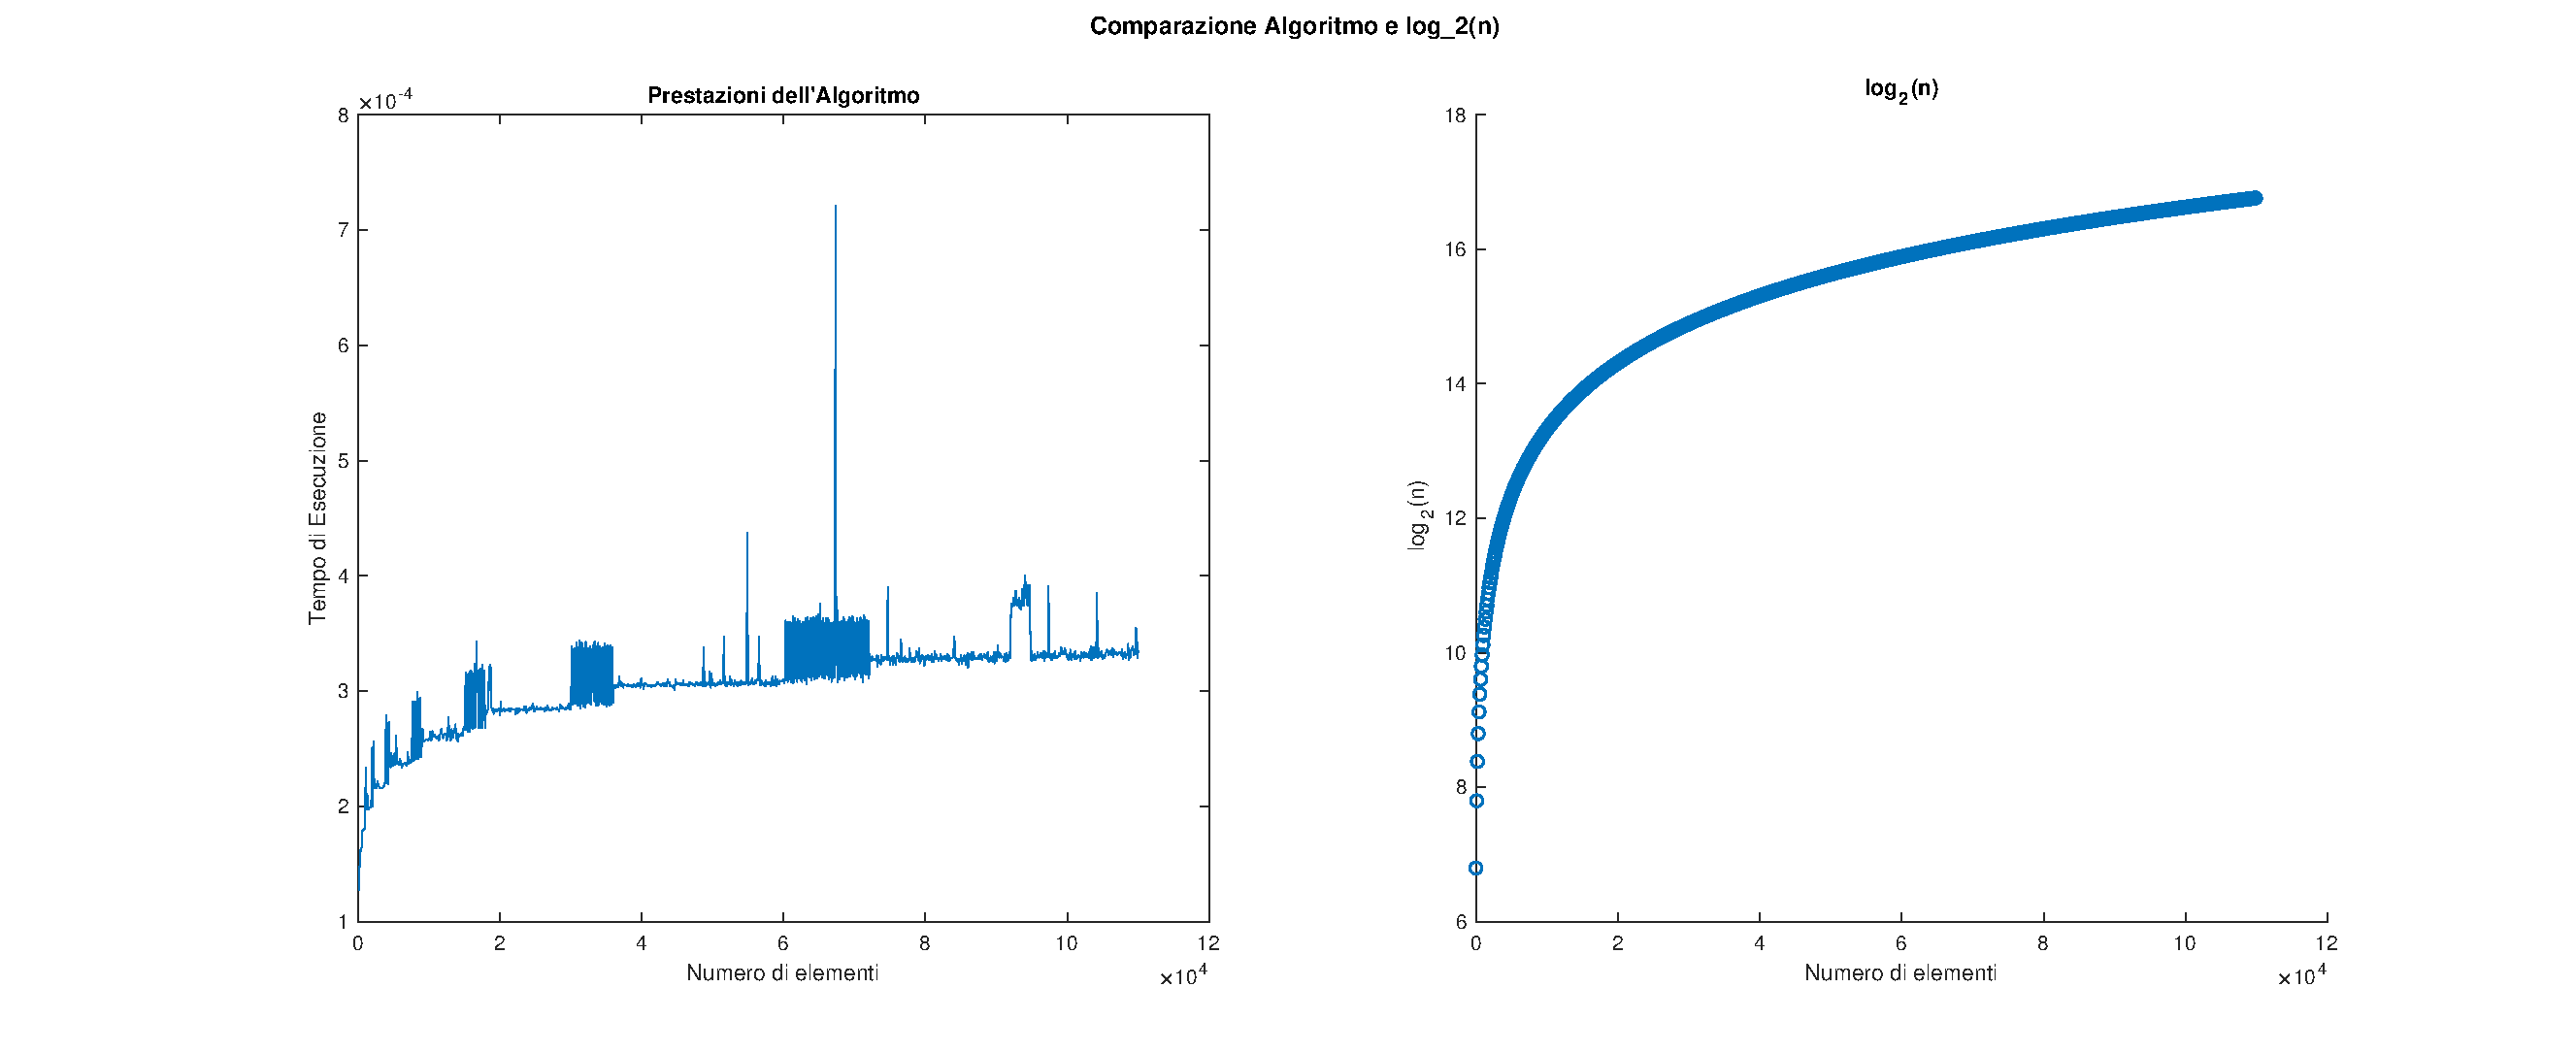
\includegraphics[width=\textwidth,height=\textheight,keepaspectratio]{./TeX_files/chart/comparison}
    \caption{Grafico che mette a confronto numero di elementi/tempo di esecuzione e  numero di elementi/$log_2$(\#elementi)}
\vspace{-10pt}
\end{figure}

